\chapter{Intégration sur un segment des fonctions à valeurs réelles} % (fold)

\begin{tcolorbox}
Requirements : Continuité

Last update : \textit{13 Septembre, 2023}, Shanghai
\end{tcolorbox}

\section{Continuité Uniforme (Révision)} % (fold)
\label{sec:Continuité Uniforme (Révision)}

% subsection Continuité Uniforme (Révision) (end)
\subsection{Fonctions uniformément continues} % (fold)
\label{sub:Fonctions uniformément continues}
\begin{Definition}[colbacktitle=red!75!black]{Fonction uniformément continue}{}
Soit $f:I \to \mathbb{R}$, $f$ est \textbf{uniformément continue} lorsque 
\begin{equation}
  \forall \varepsilon>0, \; \exists \eta >0,\; {\color{red} \forall} (x, y) \in I ^{2}, \;| x- y| \le \eta  \implies |f(x) - f(y)| \le \varepsilon
\end{equation}
\end{Definition}

\begin{Prop}{Lipschitz, uniformément continue, continue}{}
Soit $f : I \to \mathbb{R}$, donc : $f$ lipschitizenne $\implies$ $f$ uniformément continue $\implies$ $f$ continue.
\end{Prop}

\subsection{Théorèm de Heine} % (fold)
\label{sub:}

% subsection  (end)
\label{Thm: Heine}
\begin{Theorem}{Théorème de Heine}{}
Une fonction \underline{continue} sur un \underline{segment} est uniformément continue sur ce segment.
\end{Theorem}

\section{Fonctions en escaliers} % (fold)
\label{sec:Fonctions en escaliers}

\subsection{Subdivision d'un segment} % (fold)
\label{sub:Subdivision d'un segment}

\begin{Definition}[colbacktitle=red!75!black]{Subdivision}{}
  Une \textbf{subdivision} de $[a,]$ est une suite finie $\sigma = (a_k) _{k \in [\![0,n]\!]}$ strictement croissante avec $a_0 = a$ et $a_n = b$. On peut alors écrire :
  \begin{equation}
    a = a_0 < a_1 < a_2 < \dots <a _{n-1} < a_n = b
  \end{equation}
\end{Definition}





\subsection{Fonctions en escaliers} % (fold)
\label{sub:Fonctions en escaliers}

\begin{Definition}[colbacktitle=red!75!black]{Fonction en escalier}{}
  On appelle \textbf{fonction en escalier} sur $[a,b]$ toute fonction $\varphi$ définie sur $[a,b]$ pour laqulle il existe une subdivision $\sigma = (a_k) _{k \in [\![0, n]\!]}$ de $[a,b]$ vérifiant 
  \begin{equation}
    \forall k\in [\![1, n]\!],\; \exists \lambda_k \in \mathbb{R},\; \forall x\in ]a _{k-1}, a_k[, \; \varphi(x) = \lambda_k
  \end{equation}
\end{Definition}

Remarque : La subdivision $\sigma$ introduite eset \textbf{subordonnée} à $\varphi$




\subsection{Intégrale d'une fonction en escalier} % (fold)
\label{sub:Intégrale d'une fonction en escalier}

\begin{Definition}[colbacktitle=red!75!black]{Intégrale d'une fonction en escaliers}{}
\begin{equation}
  \int_{[a,b]}^{} \varphi = \sum_{k=0}^{n-1} c_k (x _{k+1} - x_k)
\end{equation}
\end{Definition}

\subsection{Propriétés de l'intégrale d'une fonction en escaliers} % (fold)
\label{sub:Propriétés de l'intégrale d'une fonction en escaliers}
Linéarité

% subsection Propriétés de l'intégrale d'une fonction en escaliers (end)

% subsection Intégrale d'une fonction en escalier (end)
% subsection Fonctions en escaliser (end)
% subsection Subdivision d'un segment (end)
% section Fonctions en escaliers (end)
\section{Fonctions continues par morceaux} % (fold)
\label{sec:Fonctions continues par morceaux}

\subsection{Définitions et propriétés} % (fold)
\label{sub:Définitions et propriétés}

% subsection Définitions et propriétés (end)
\begin{Definition}[colbacktitle=red!75!black]{Fonction continue par morceaux sur un segment}{}
  Soit $[a,b]$ un segment. $\varphi : [a,b] \to \mathbb{R}$ est \textbf{continue par morceaux} sur $[a,b]$ lorsqu'il \underline{existe une subdivision} $\tau$ du segment telle que 
  \begin{itemize}

    \item $\forall k \in [\![0, n-1]\!]$, $\varphi| _{]x_k, x _{k+1}[}$ est continue
      
    \item $\varphi | _{]x_k, x _{k+1}[}$ est prolongeable par continuité sur $]x_k, x _{k+1}[$. 

  \end{itemize}
  Une telle subdivision est dite \textbf{adaptée} ou \textbf{subordonnée} à $\varphi$.

  \begin{figure}[H] %h:当前位置, t:顶部, b:底部, p:浮动页
    \centering
    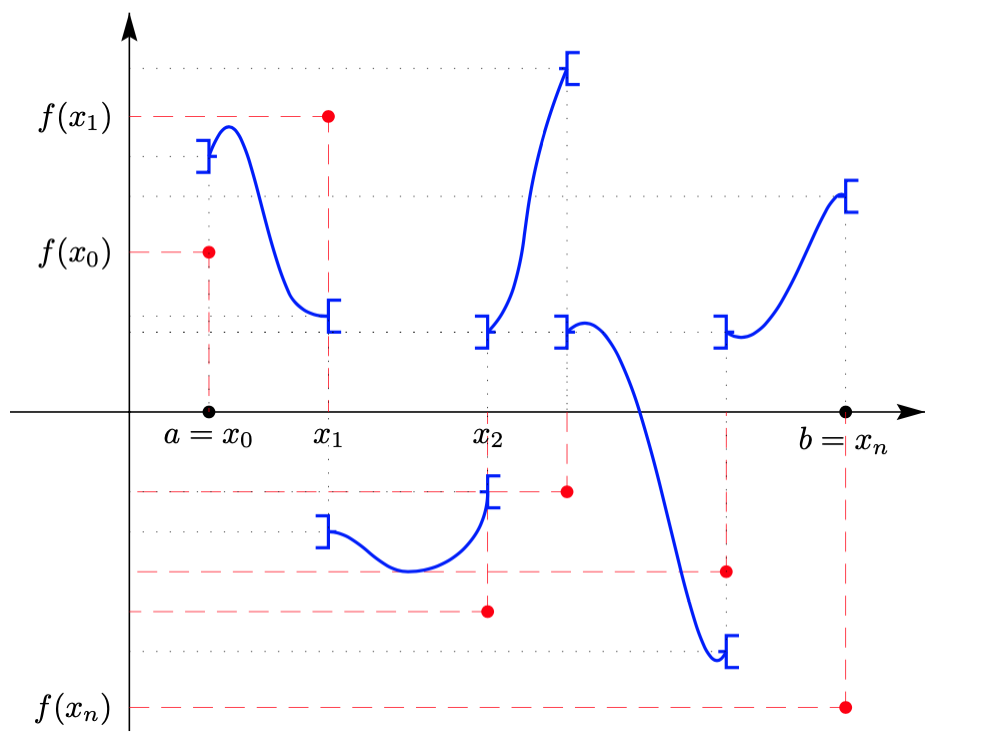
\includegraphics[width=0.6\textwidth]{./assets/Fonction continue par morceaux sur un segment.png}
    \caption{Fonction continue par morceaux sur un segment}
    \label{fig:Fonction continue par morceaux sur un segment}
  \end{figure}

  

\end{Definition}

Toute fonction en escalier sur $[a,b]$ est \textbf{continue par morceaux} sur $[a,b]$.

\begin{Prop}{Bornée d'une fonction continue par morceaux}{}
  Soit $\varphi$ est une fonction \textbf{continue par morceaux} sur $[a,b]$ donc elle est bornée.
\end{Prop}

\begin{myproof}{}{}
  Soit $f$ fonction continue, pour chaque $i \in [\![0, k-1]\!]$, $\bar{f}_i$ la fonction \underline{continue} prolongé défini sur \underline{un segment} $[x_i, x _{i+1}]$ pour chaque petit intervalle. Donc elle est bornée.
\end{myproof}

\begin{Prop}{}{}
  L'ensemble des fonctions réelles \textbf{continues par morceaux} sur $[a,b]$ est un \underline{sous-espace vectoriel} de $\mathcal{F}([a,b], \mathbb{R})$
\end{Prop}

\subsection{Approximation des fonctions par morceaux par les fonctions en escalier} % (fold)
\label{sub:Approximation des fonctions par morceaux par les fonctions en escalier}

\begin{Theorem}{Approximation d'une fonction continue par une fonction en escalier}{}
  Soit $f$ une fonction continue sur le segment $[a,b]$ et $\varepsilon>0$. 

  Donc, il existe une fonction en escalier $\varphi$ telle que 
  \[
    \| f- \varphi \| _{\infty}  = \sup _{x \in [a,b]} |f(x) - \varphi(x)|\le \varepsilon
  \]

  \begin{figure}[H] %h:当前位置, t:顶部, b:底部, p:浮动页
    \centering
    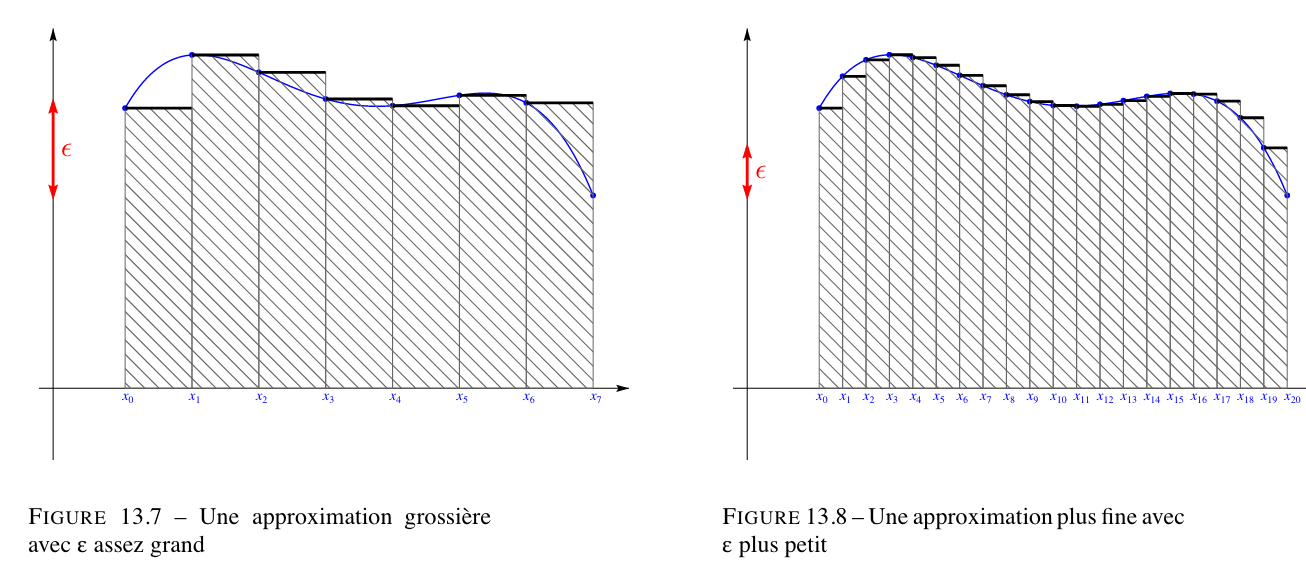
\includegraphics[width=0.8\textwidth]{./assets/Approximation d'une fonction 1.png}
    \caption{Approximation d'une fonction continue}
  \end{figure}

  
\end{Theorem}

\begin{myproof}{}{}
  $f$ est continue sur le segment, donc uniformément continue. (Théorème de Heine \ref{Thm: Heine}) Dans l'écriture $\varepsilon - \eta$, prenons $h = (b-a)/n \le \varepsilon$, construisons :
  \begin{equation}
    x_i = a + ih,\; \forall x \in [x_i,x _{i+1}[ , \; \varphi(x) = f(x_i),\; \varphi(b) = f(b)
  \end{equation}
\end{myproof}


\begin{Lenma}{Décomposition d'une fonction continue par morceaux}{}
  Soit $f$ une fonction continue par morceaux sur le gement $[a,b]$. 

Il existe 
\begin{itemize}

  \item une fonction $g$ continue sur $[a,b]$ 
  \item une fonction $\psi$ en escalier sur $[a,b]$

\end{itemize}
telles que $f = g + \psi$
  \begin{figure}[H] %h:当前位置, t:顶部, b:底部, p:浮动页
    \centering
    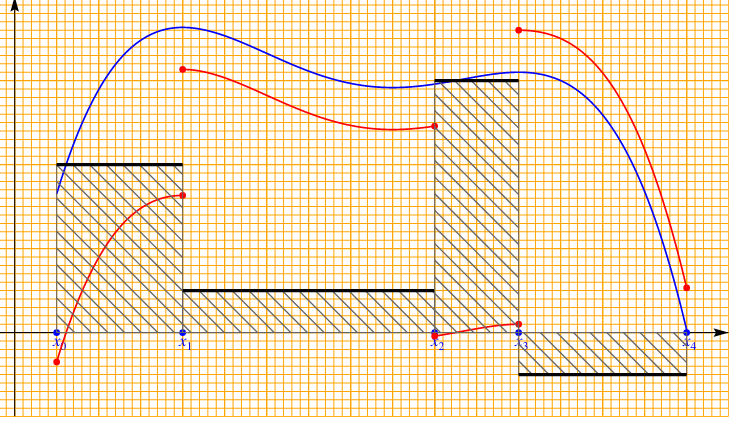
\includegraphics[width=0.6\textwidth]{./assets/Approximation d'une fonction 2.png}
    \caption{Décomposition d'une fonction continue par morceaux}
  \end{figure}
\end{Lenma}


\begin{Corollary}{Approximation uniforme d'une fonction continue par morceaux par une foncution en escalier}{}
  Soit $f$ une fonction continue par morceaux sur le segment $[a,b]$ et $\varepsilon>0$. Il existe $\varphi$ en escalier sur $[a,b]$ telle que $\| f-\varphi \| _{\infty} \le \varepsilon$.
\end{Corollary}
\begin{myproof}{}{}
Soit $f  = g + \psi$, $\exists \xi$ telle que $\| g - \xi \| _{\infty} \le \varepsilon$, notons $\varphi = \psi + \xi$, $\| f - \varphi \| _{\infty} = \| g - \xi \| _{\infty} \le \varepsilon$
\end{myproof}

\begin{Corollary}{Encadrement d'une fonction continue par morceaux par deux fonctions en escalier}{}
  Soit $f$ une fonction continue par morceaux sur le segment $[a,b]$ et $\varepsilon>0$. $\exists \varphi, \psi \in \mathcal{E}([a,b], \mathbb{R})$ vérifiant :
  \begin{itemize}

      \item $\varphi \le f \le \psi$ 
      \item $\| \psi - \varphi \| _{ \infty} \le \varepsilon$

  \end{itemize}
\end{Corollary}





\subsection{Intégrale d'une fonction continue par morceaux} % (fold)
\label{sub:Intégrale d'une fonction continue par morceaux}

\begin{Prop}{Intégrale de Riemann d'une fonction continue par morceaux}{}
  Soit $f$ continue par morceaux sur $[a,b]$. Les ensembles 
\begin{gather}
  I _{<f} = \left\{ \int _{[a,b]} \varphi,\; \varphi \in \mathcal{E}([a,b],\mathbb{R}), \; \varphi \le f\right\} \\
  I _{>f} = \left\{ \int _{[a,b]} \varphi,\; \varphi \in \mathcal{E}([a,b],\mathbb{R}), \; \varphi \ge f\right\}
\end{gather}

On a 
\begin{itemize}

    \item $I _{<f}$ admet une borne supérieur
    \item $I _{>f}$ admet une borne inférieur
    \item $\sup I _{<f} = \inf I _{>f}$
    

\end{itemize}


\end{Prop}

\begin{Definition}[colbacktitle=red!75!black]{Intégrale de Riemann}{}
  L'\textbf{intégrale de Riemann} de la fonction continue par morceaux $f$ sur $[a,b]$ par : 
  \begin{equation}
    \int _{[a,b]} f = \sup I _{<f} = \inf I _{>f}
  \end{equation}

\end{Definition}


\begin{note}{}{}
Pour montrer qu'une fonction $f$ est \textbf{intégrable sur un segment}, il suffit de montrer que $f$ est \underline{continue par morceaux sur ce segment}.
\end{note}

\subsection{Propriétés de l'intégrale} % (fold)
\label{sub:Propriétés de l'intégrale}

\begin{Theorem}{Forme linéaire}{}
L'intégrale est une \underline{forme linéaire} sur l'{espace vectoriel des fonctions continues par morceaux}.
\end{Theorem}



\begin{Prop}{L'intégrale d'une fonction continue par morceaux positive}{}
  Soit $\varphi$ continue par morceaux sur $[a,b]$. Alors, 
  \begin{equation}
    \forall x \in [a,b], \; \varphi(x) \ge 0 \implies \int _{[a,b]} \varphi_1  \ge 0
  \end{equation}
\end{Prop}

\begin{Corollary}{}{}
\begin{equation}
  \varphi_1 \le \varphi_2 \implies \int _{[a,b]} \varphi_1 \le \int _{[a,b]} \varphi_2
\end{equation}
\end{Corollary}

\begin{Prop}{Relation de Chasles}{}
\begin{equation}
  \int_{[a,b]}f = \int_{[a,c]}^{} f + \int_{[c,b]}^{}f
\end{equation}
\end{Prop}



\subsection{Majorations fondamentales} % (fold)
\label{sub: Majorations fondamentales} % (fold)

\begin{Theorem}{}{}
  Soient $f$ une fonction réelle continue par morceaux sur le segment $[a,b]$. Donc, il existe $(m, M) \in \mathbb{R}^{2}$ tels que $\forall x \in [a,b]$, $m \le f(x) \le M$. donc, 
  \begin{equation}
    \boxed{m(b-a) \le \int _{[a,b]} f(x) \mathrm{d} x \le M(b-a)}
  \end{equation}

  \begin{figure}[H] %h:当前位置, t:顶部, b:底部, p:浮动页
    \centering
    \includegraphics[width=0.5\textwidth]{./assets/Encadrement d'une intégrale.png}
    \caption{Encadrement d'une intégrale}
    \label{fig:Encadrement d'une intégrale.png}
  \end{figure}
\end{Theorem}

\begin{Theorem}{Inégalité triangulaire intégral}{}
  Soit $f$ une fonction continue par morceaux sur le segment $[a,b]$. Donc, $f$ est bornée sur $[a,b]$ et 
  \begin{equation}
    \boxed{\left|\int_{a}^{b} f(x) \mathrm{d}x\right| \le \int_{a}^{b} |f(x)| \mathrm{d} x \le (b-a) \sup _{[a,b]}|f|}
  \end{equation}
\end{Theorem}

\begin{myproof}{}{}
$- |f| \le f \le |f|| \implies - \int_{}^{}|f| \le \int_{}^{}f \le \int_{}^{}|f| $.
\end{myproof}

\begin{Theorem}{Inégalité de la moyenne}{}
  Soient $f,g$ continues par morceaux sur $[a,b]$. Alors, 
  \begin{equation}
    \left| \int_{[a,b]}^{} fg\right| \le \sup _{[a,b]} |f| \int_{[a,b]}^{}|g|
  \end{equation}
\end{Theorem}

\begin{Theorem}{Inégalité de Cauchy-Schwarz}{}
  Soient $f$ et $g$ continues sur le segment $[a,b]$. Notons $\|f \|_2 = \sqrt{\int_{[a,b]}^{}f ^{2}(x) \mathrm{d}x}$, on obtient 
  \begin{equation}
    \langle fg \rangle \le\| f \|_2 \| g \|_2 \implies\boxed{\left| \int_{[a,b]}^{}fg \right| \le \sqrt{\int_{[a,b]}^{}f ^{2}} \sqrt{\int_{[a,b]}^{}g ^{2}}}
  \end{equation}
\end{Theorem}

\begin{myproof}{}{}
D'après la positivité de 
\begin{equation}
  P = \int_{[a,b]}^{}(f+\alpha g) ^{2}
\end{equation}
\end{myproof}

\begin{Theorem}{Inégalité de Minkowski}{}
  Soient $f$ et $g$ continues sur le segment $[a,b]$. Notons $\|f \|_2 = \sqrt{\int_{[a,b]}^{}f ^{2}(x) \mathrm{d}x}$, on obtient 
  \begin{equation}
    \| f+g \|_2 \le \| f \|_2 + \| g \|_2
  \end{equation}
\end{Theorem}

\begin{myproof}{}{}
  Développer $\int_{[a,b]}^{}(f+g) ^{2}$ et utilisons Cauchy-Schwarz.
\end{myproof}











% subsection  (end)


% subsection Propriétés de l'intégrale (end)







% subsection Intégrale d'une fonction continue par morceaux (end)





% subsection Apptoximation des fonctions par morceaux par les fonctions en escalier (end)






% section Fonctions continues par morceaux (end)

\section{Primitive et intégrale d'une fonction continue} % (fold)

\subsection{Définitions} % (fold)
\label{sub:Définitions}

% subsection Définitions (end)

\begin{Definition}[colbacktitle=red!75!black]{Primitive}{}
Soit $f : I \to \mathbb{R}$ définie sur un \underline{intervalle} $I$. $F : I \to \mathbb{R}$ est \textbf{primitive} de $f$ sur $I$ si et seulement si :
\begin{itemize}

    \item $F$ dérivable sur $I$ 
    \item et $\forall x \in I$, $F'(x) = f(x)$

\end{itemize}
\end{Definition}

\begin{Prop}{Deux primitives d'une même fonction}{}
  Les primitives d'une même fonction diffèrent d'une constante.

Soit $F$, $G$ primitives de $f : I \to \mathbb{R}$. Alors, $\exists c \in \mathbb{R}$, $F = G + c$
\end{Prop}

\begin{Lenma}{Continuité de la primitive}{}
Si $f : I \to \mathbb{R}$ \underline{continue par morceaux}, alors $F$ \underline{continue} sur $I$.
\end{Lenma}

\begin{myproof}{}{}
  Comme $f$ continue par morceaux sur un intervalle, donc elle est bornée.
Soient $(x, y) \in I ^{2}$, alors 
\begin{equation}
  |F(y) - F(x) | = \left| \int_{a}^{y} f(t) \mathrm{d} t - \int_{a}^{x} f(t) \mathrm{d} t \right| \le \int_{x}^{y} |f(t) | \mathrm{d} t \le \sup _{x \in [a,b]} |f(x)| |y-x|
\end{equation}
donc lipschitizenne, donc continue.
\end{myproof}

\subsection{TFA} % (fold)
\label{sub:TFA}

% subsection TFA (end)
\begin{Theorem}{\color{red} Théorème fondamental de l'analyse (TFA)}{}
Soit $f$ continue sur un intervalle $I$ de $\mathbb{R}$, soit $a \in I$. 

Alors, la fonction $F : I \to \mathbb{R}$
\begin{equation}
  F : x \mapsto \int_{a}^{x} f(t) \mathrm{d}t
\end{equation}
est de classe $\mathscr{C} ^{1}$ sur $I$ et est \underline{la seule primitive de $f$ qui s'annule en $a$} : 
\begin{equation}
  F' = f,\quad F(a) = 0
\end{equation}
\end{Theorem}

\begin{Corollary}{}{}
Une fonction continue sur un intervalle de $\mathbb{R}$ \underline{possède une primitive} sur $I$.
\end{Corollary}

\begin{Corollary}{Calcul d'intégrale}{}
  Soit $f : I \to \mathbb{R}$ continue sur le \underline{segment} $[a,b] \subset I$. Soit $G$ une primitive de $f$ (c'est-à-dire, $G_c = F + c$). Alors  l'\textbf{intégrale} de $F$ sur $[a,b]$ est :
  \begin{equation}
    \int_{a}^{b} f(t) \mathrm{d} t = G(b) - G(a)
  \end{equation}
\end{Corollary}

\begin{Theorem}{\color{red} TFA (deuxième forme)}{}
Soit $f$ une fonction de classe $\mathcal{C} ^{1}$ sur $I$ de $\mathbb{R}$, soit $(a,b) \in I ^{2}$, on a :
\begin{equation}
  f(b) - f(a) = \int_{a}^{b} f'(t) \mathrm{d} t
\end{equation}
\end{Theorem}

\begin{note}{}{}
  Quand on a une hypothèse sur $f'$, et je souhaite de svaoir $f$.
\end{note}


\begin{Example}{L'inégalité de Poincaré}{}
  Soit $E = \{ f \in \mathcal{C} ^{1}([a,b], \mathbb{R}), \; f(a) = 0\}$. $\exists C \ge 0$ telle que 
  \begin{equation}
    \forall f \in E, \; \| f \| _{2} \le C \| f' \|_2
  \end{equation}

\end{Example}

\begin{myproof}{}{} Soit $x \in [a,b]$
\begin{gather}
  f(x) = f(a) + \int_{a}^{x} f'(t) \mathrm{d} t = \int_{a}^{x} f'(t) \mathrm{d}t \\ 
  (\text{Cauchy-Schwarz})\implies f ^{2}(x) \le \int_{a}^{x} 1 ^{2} \mathrm{d} t \int_{a}^{x} f^{'2}(t) \mathrm{d} t \le (x-a) \int_{a}^{b} f ^{'2}(t) \mathrm{d} t \\ 
  \int_{a}^{b} f ^{2}(t)  \mathrm{d} t \le \int_{a}^{b}f ^{'2}(t) \mathrm{d}t \times \int_{a}^{b}(x-a) \mathrm{d}x  = \frac{(b-a) ^{2}}{2}  \int_{a}^{b} f ^{'2}(t) \mathrm{d} t \implies C = \frac{b-a}{\sqrt{2}} 
\end{gather} 
\end{myproof}

\begin{Theorem}{Dérivée d'une fonction définie par une integrale}{}
Soit $f$ continue sur $I$, $u, v : J \to I$ dérivables sur $J$. Alors, $G : J \to \mathbb{R}$ définie au-dessous est dérivable sur $J$ :
\begin{equation}
  G : x \mapsto \int_{u(x)}^{v(x)} f(t) \mathrm{d} t, \quad G'(x) = v'(x) f[v(x)] - u'(x) f[u(x)]
\end{equation}



\end{Theorem}

\begin{myproof}{}{}
\begin{equation}
  G(x) = \int_{a}^{v(x)} f(t) \mathrm{d}(t) - \int_{a}^{u(x)} f(t) \mathrm{d}(t) = F(v(x)) - F(u(x)) \implies G = F \circ v - F \circ u
\end{equation}
\end{myproof}

\begin{Example}{}{}
  Variations de la fonction : $g : ]1, + \infty[ \to \mathbb{R}$:
\begin{equation}
  g : x \mapsto \int_{x}^{x ^{2}} \frac{\mathrm{d}t}{t ^{2}-1} 
\end{equation}
\end{Example}

\begin{myproof}{}{}
\begin{equation}
  g'(x) = 2x f(x ^{2}) - f(x) \text{ avec} f : x \mapsto \frac{1}{x ^{2} - 1} 
\end{equation}
Donc s'annule en $x_0 = 1 + \sqrt{2}$, croissante sur $]1, x_0]$ et décorissante sur $[x_0, + \infty[$
\end{myproof}

\subsection{Valeur moyenne} % (fold)
\label{sub:Valeur moyenne}

\begin{Theorem}{Valeur moyenne d'une fonction continue}{}
  Soit $f \in \mathcal{C}([a,b], \mathbb{R})$, il existe $c \in [a,b]$ tel que 
  \begin{equation}
    \frac{1}{b-a}  \int_{a}^{b} f(t) \mathrm{d}t = f(c)
  \end{equation}
\end{Theorem}


% subsection Valeur moyenne (end)
\section{Calcul de primitives et d'intégrales} % (fold)
\label{sec:Calcul de primitives et d'intégrales}

\subsection{IPP} % (fold)
\label{sub:IPP}

\begin{Prop}{Méthode d'intégration par partie (IPP)}{}
Soit $u$ et $v$ des fonctions de classe $\mathcal{C} ^{1}$ sur intervalle $I$ de $\mathbb{R}$, donc :
\begin{equation}
  \int_{a}^{b} u'(t) v(t) \mathrm{d} t = [u(t)v(t)]_a ^{b} - \int_{a}^{b} u(t)v'(t) \mathrm{d}t
\end{equation}
\end{Prop}

\subsection{Changement de variable} % (fold)
\label{sub:Changement de variable}
\begin{Prop}{
    Changement de variable
  }{}
\begin{equation}
  \int_{\varphi(a)}^{\varphi(b)} f(t) \mathrm{d}t = \int_{\alpha}^{\beta} f(\varphi(u)) \varphi'(u) \mathrm{d}u = \int_{\alpha
  }^{\beta} f(\varphi(u)) \mathrm{d}(\varphi(u))
\end{equation}
\end{Prop}


% subsection Changement de variable (end)



% subsection IPP (end)
% section Calcul de primitives et d'intégrales (end)












\section{Formules de Taylor} % (fold)
\label{sec:Formules de Taylor}

\subsection{Formule de Taylor avec reste intégral} % (fold)
\label{sub:Formule de Taylor avec reste intégral}

\begin{Theorem}{Formule de Taylor avec reste intégral}{}
Soit $f$ une fonction de classe $\mathscr{C} ^{n+1}$ sur un intervalle $I$ de $\mathbb{R}$. 
\begin{equation}
  f(x) = \sum_{k=0}^{n} \frac{f ^{(k)}(a)}{k!} (x-a) ^{k} + \int_{a}^{x} \frac{(x-t) ^{n}
  }{n!}  f ^{(n+1)}(t) \mathrm{d}t
\end{equation}

\begin{itemize}

    \item \textbf{Polynôme de Taylor de $f$} de degré $n$ : 
      \begin{equation}
        T_n(x) = f(a) + \frac{x-a}{1!} f'(a) + \dots + \frac{(x-a) ^{n}}{n!} f ^{(n)}(a)
      \end{equation}

    \item \textbf{Reste intégral} : 
      \begin{equation}
        R_n(x) = \int_{
          a
        }^{x} \frac{(x-t) ^{n}}{n!} f ^{(n+1)} (t) \mathrm{d} t
      \end{equation}
\end{itemize}
\end{Theorem}

  \begin{note}{}{}
 L'idée principal : 
 \begin{itemize}

     \item TFA(2)
    \item IPP

 \end{itemize}
  \end{note}
\begin{myproof}{}{}


  

Si la fonction $f$ de classe $\mathscr{C} ^{1}$, on sait que 
\begin{equation}
  f(x) = f(a) + \int_{a}^{x} f'(t) \mathrm{d} t
\end{equation}

Faisons une IPP à la dernière terme, et supposons que $f$ de classe $\mathscr{C} ^{2}$. Donc, en admettant que 
\begin{equation}
  f(x) = f(a) + [tf'(t)] _a ^{x} - \int_{a}^{x} tf"(t) \mathrm{d}t = f(a) + xf'(x) - af'(a) - \int_{a}^{x} tf"(t) \mathrm{d}t
\end{equation}

On ne sait pas $f'(x)$. Maintenant, considérons la primitive de $g : t \mapsto 1$ s'annule en $x$

\begin{equation}
  f(x) = f(a) + [-(x-t)f'(t)] _a ^{x} + \int_{a}^{x}(x-t) f"(t) \mathrm{d}t = f(a) + (x-a) f'(a) + \int_{a}^{x} (x-t) f"(t) \mathrm{d}t
\end{equation}

Ensuite, une simple récurrence.
\end{myproof}

\subsection{Inégalité de Taylor-Lagrange} % (fold)
\label{sub:Inégalité de Taylor-Lagrange}

\begin{Theorem}{\color{red} Inégalité de Taylor-Lagrange}{}
  Dans la formule \ref{sub:Formule de Taylor avec reste intégral}, on a $f = T_n + R_n$ : 
  \begin{equation}
  f(x) = \sum_{k=0}^{n} \frac{f ^{(k)}(a)}{k!} (x-a) ^{k} + \int_{a}^{x} \frac{(x-t) ^{n}
  }{n!}  f ^{(n+1)}(t) \mathrm{d}t
  \end{equation}


On a alors, 
  \begin{equation}
    |R_n(x) | \le \frac{|x-a| ^{n+1}}{(n+1)!} \sup _{t \in [a,x]} |f ^{(n+1)}(t)|
  \end{equation}

\end{Theorem}

\begin{myproof}{}{}
  Utiliser les téchniques dans \ref{sub: Majorations fondamentales}
\end{myproof}


\subsection{Formule de Taylor-Young} % (fold)
\label{sub:Formule de Taylor-Young}

\begin{Theorem}{\color{red} Formule de Taylor-Young}{}

  Soient $f$ de classe $\mathscr{C} ^{n}$. Dans la formule \ref{sub:Formule de Taylor avec reste intégral}, on a $f = T_n + R_n$. Il existe une fonction $\varepsilon (x)  \underset{x \to a}{\longrightarrow} 0$ telle que 
  \begin{equation}
    \forall x \in I, \; f(x) = T_n(x) + (x-a) ^{n}\varepsilon(x)
  \end{equation}
\end{Theorem}

\begin{myproof}{}{}
\begin{itemize}

  \item Si $f$ de classe $\mathscr{C} ^{n+1}$, d'après le théorème \ref{sub:Inégalité de Taylor-Lagrange}, on trouve $\frac{|R_n(x)|}{|x-a| ^{n}} \to 0$.

\end{itemize}
\end{myproof}

\subsection{Utilisation des trois formules de Taylor} % (fold)

\begin{itemize}

    \item La \textbf{formule de Taylor-intégrale} est la plus précise, et les deux autres formules en sont une conséquence. 
    \item \textbf{Formule de Taylor-Young} donne une \underline{approximation locale} au voisinage d'un point $a$. 
    \item \textbf{Inégalité de Taylor-Lagrange} fournit une \underline{majoration globale} du reste $R_n$ de cette approximation sur un segment $[a,x]$.

\end{itemize}
\section{Méthode des rectangles, Sommes de Riemann} % (fold)
\label{sec:Méthode des rectangles, Sommes de Riemann}

\begin{Theorem}{Méthode des rectangles}{}
\begin{itemize}

  \item Approximation d'intégrale. Soit $f$ de classe $\mathscr{C} ^{1}$ sur $[a,b]$. 
    \begin{itemize}

        \item On effectue une subdivison du segment $[a,b]$ de pas constant $h = (b-a) / n$. 

      \item On pose pour chaque $k \in [\![0, n]\!]$, $x_k = a + kh$. 
      \item Posons 
        \begin{equation}
          R_n = h.(f(x_1) + \dots + f(x_n)) = \frac{b-a}{n}  \sum_{k=0}^{n-1} f(x_k)
        \end{equation}

    \end{itemize}

  \item Majoration de l'erreur.  Suposons que $I$ l'intégrale de la fonction $f$.
    \begin{equation}
      |I - R_n| \le \frac{(b-a) ^{2}}{2n} \| f' \| _{\infty}
    \end{equation}

\end{itemize}
\end{Theorem}

\begin{myproof}{}{}
Pour chaque segment, l'erreur : 
\begin{gather}
  \varepsilon _{n,k} = \left| \int_{x_k}^{x _{k+1}} f(t) \mathrm{d} t - \frac{b-a}{n} f(x_k) \right| \le \int_{x_k}^{x _{k+1}} |f(t) - f(x_k) | \mathrm{d} t \\ 
  |f(t) - f(x_k) | = \left| \int_{x_k}^{t} f'(t) \mathrm{d} t \right| \le \sup _{[x \in [a,b]]}|f'(x)| ( t- x_k) \\ 
  |\varepsilon _{n,k}|\le \| f' \| _{\infty} \frac{(x _{k+1} - x_k) ^{2}}{2} = \| f' \| _{\infty}  \frac{(b-a) ^{2}}{2 n ^{2}} 
\end{gather}
\end{myproof}

\begin{Theorem}{\color{red} Convergence d'une somme de Riemann}{}
  Soit $f$ continue sur le \underline{segment} $[0,1]$, on a 
\begin{gather}
  R_n = \frac{1}{n} \sum_{k=0}^{n-1} f \left( \frac{k}{n}  \right)  \underset{n \to + \infty}{\longrightarrow}  \int_{0}^{1} f(x) \mathrm{d} x \\ 
  T_n = \frac{1}{n} \sum_{k=1}^{n} f \left( \frac{k}{n}  \right)  \underset{n \to + \infty}{\longrightarrow}  \int_{0}^{1} f(x) \mathrm{d} x
\end{gather}

Plus généralement, si $f$ une fonction continue sur le segment $[a,b]$, et si $\xi_k \in [a+kh, a+ (k+1)h]$, on a 
\begin{equation}
  u_n = \frac{b-a}{n}  \sum_{
    k=0
  }^{n-1} f(\xi_k)  \underset{n \to + \infty}{\longrightarrow}  \int_{a}^{b} f(x) \mathrm{d}x
\end{equation}
\end{Theorem}

\begin{myproof}{}{}
\begin{itemize}

    \item Si $f \in \mathscr{C} ^{1}$, d'après le théorème précédante. 
    \item Si $f$ est uniquement continue. 
      \begin{itemize}

          \item Montrons que $\| f - \varphi_n \| _{\infty}  \underset{n \to \infty}{\longrightarrow} 0$ (Théorème de Heine - Importance d'un segment !!) 

          \item  Donc, 
            \begin{equation}
              |I - R_n | \le \int_{0}^{1} | f(t)- \varphi_n(t) |\mathrm{d} t  \le \| f - \varphi_n \| _{\infty}  \underset{n \to \infty}{\longrightarrow} 0
            \end{equation}

      \end{itemize}

\end{itemize}
\end{myproof}


\begin{Example}{}{}
Limite de suite 
\begin{equation}
  u_n = \sum_{p=n}^{2n-1} \frac{1}{2p+1}   \underset{n \to + \infty}{\longrightarrow} \frac{\ln(2)}{2} 
\end{equation}
\end{Example}





% section Méthode des rectangles, Sommes de Riemann (end)

% section Utilisation des trois formules de Taylor (end)


% subsection Formule de Taylor-Young (end)



% subsection Inégalité de Taylor-Lagrange (end)
% subsection Formule de Taylor avec reste intégral (end)
% section Formules de Taylor (end)

% section  (end)
% chapter Intégration (end)
